\documentclass{beamer}
\usepackage{graphicx}
\usepackage{tikz}
\usetikzlibrary{shapes,arrows}
\usepackage{tikz}
\usetheme{default}
%\usecolortheme{seahorse}
\usepackage{default}
\usepackage[makeroom]{cancel}

  \setbeamertemplate{footline}[page number]
\setbeamertemplate{navigation symbols}{}
\setbeamertemplate{frametitle}[default][center]
\setbeamerfont{frametitle}{shape=\scshape}

\usepackage{color}
\usepackage{multirow}

\usepackage{media9}%
\newcommand{\includemovie}[3]{%
\includemedia[%
width=#1,height=#2,%
activate=pagevisible,%
deactivate=pageclose,%
addresource=#3,%
flashvars={%
src=#3 % same path as in addresource!
&autoPlay=true % default: false; if =true, automatically starts playback after activation (see option ?activation)?
&loop=true % if loop=true, media is played in a loop
&controlBarAutoHideTimeout=0 %  time span before auto-hide
}%
]{}{StrobeMediaPlayback.swf}}%


{\title{\textsc{Numerical Methods-Lecture XII: \\ CGE Modelling} \\ \ \\ \tiny (See Harberger 1962, Shoven \& Whalley 1984, Gallen \& Mulligan 2016)}
\author{Trevor Gallen}
\date{}

\begin{document}

\begin{frame}
\titlepage
\end{frame}


%\begin{frame}
%\frametitle[alignment=center]{Agenda}
%\begin{itemize}
%\item Mike Powell
%\item Stanton
%\item Code from Sargent \& Ljungqvist
%\item NCG
%\begin{itemize}
%\item Functional forms
%\item Calibration
%\end{itemize}
%\item Solution method
%\item Model meets data
%\end{itemize}
%\end{frame}


\begin{frame}
\frametitle[alignment=center]{Harberger 1962: Motivation}
\begin{itemize}
\item Federal Insurance Contributions Act funds Social Security \& Medicare
\bigskip
\item In 2015, 7.65\% employer, 7.65\% employee
\bigskip
\item Every so often, a temporary cut or permanent hike
\bigskip
\item Example: in 2010 and 2011, FICA employee portion reduced to 5.65\%
\bigskip
\item Who benefits?
\end{itemize}
\end{frame}

\foreach \x in {1,...,4}{
\begin{frame}
\frametitle[alignment=center]{Harberger 1962: Motivation}
\includegraphics[scale=0.5]{TI_Fig\x.png}
\end{frame}
}

\begin{frame}
\frametitle[alignment=center]{Harberger 1962}
\begin{itemize}
\item Incidence is important
\bigskip
\item What if we had two industries, two types of labor?
\bigskip
\item Labor demand for one depends on labor demand for other (CES)
\bigskip
\item Free labor supply means after-tax wages must be equal within type
\bigskip
\item Harberger:
\bigskip
\begin{itemize}
\item Two factors: labor and capital
\bigskip
\item Two industries: ``corporate" and ``noncorporate"
\end{itemize}
\end{itemize}
\end{frame}

\begin{frame}
\frametitle[alignment=center]{Harberger 1962}
\Large
\begin{table}
\begin{tabular}{lcc}
 & Labor & Capital \\ 
Corporate & $L_a$ & \color<2->{red}{$K_a$}\\
Non-corporate & $L_b$ & $K_b$ \\
\end{tabular}
\end{table}
\normalsize
\begin{itemize}
\item<2-> {Who bears the incidence? Is capital harmed? Is labor harmed?\\}
\bigskip
\item<3-> {What if $K_a+K_b$, $L_a+L_b$, and $P_aY_a+P_bY_b$ stays the same?\\}
\bigskip
\item<4-> {Ans: Capital can actually benefit, labor harmed!\\}
\bigskip
\item<5-> {Why?\\}
\end{itemize}
\end{frame}

\begin{frame}
\frametitle[alignment=center]{Harberger 1962}
\begin{itemize}
\item Basic idea:
\begin{itemize}
\item Say taxed sector was heavy in untaxed input $L$
\bigskip
\item With tax, sector shrinks
\bigskip
\item As taxed sector shrinks, other sector absorbs its $K$ and $L$
\bigskip
\item Taxed sector releases little $K$ and lots of $L$
\bigskip
\item If untaxed sector can't absorb much $L$, price falls, potentially a lot
\bigskip
\item Example
\begin{itemize}
\item Taxed sector has production function $min(10L_b,K_b)$
\item Untaxed sector has production function $L_b^\alpha K_b^{1-\alpha}$
\item Elasticity of demand for taxed sector good is very high
\item For untaxed sector to absorb $L$, wages (all wages!) must decline precipitously
\end{itemize}
\end{itemize}
\end{itemize}
\end{frame}

\begin{frame}
\frametitle[alignment=center]{Harberger 1962}
\begin{itemize}
\item Harberger 1968 gave analytical formulas
\bigskip
\item Numerical examples with Cobb-Douglas and Leontief are possible
\bigskip
\item  What if we want to go further?
\bigskip
\item Want to write down a CGE model
\end{itemize}
\end{frame}

\begin{frame}
\frametitle[alignment=center]{CGE Models}
\begin{itemize}
\item Assume functional forms
\bigskip
\item Interacting agents (agent FOC's)
\bigskip
\item Markets clear
\bigskip
\item Everything adds up
\end{itemize}
\end{frame}

\begin{frame}
\frametitle[alignment=center]{CGE Models}
\begin{figure}
\centering
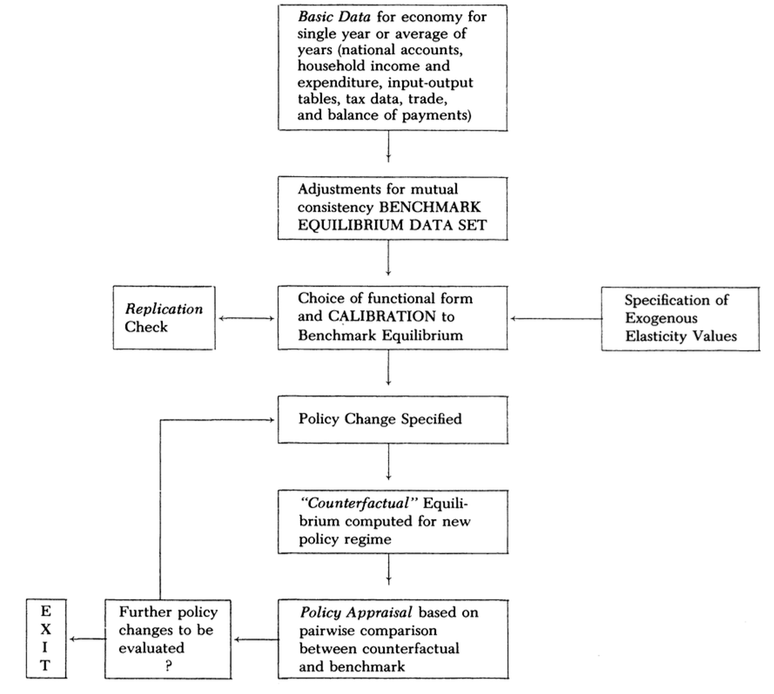
\includegraphics[scale=0.34]{Shoven_Whalley_1984.png}
\end{figure}
\end{frame}

\begin{frame}
\frametitle[alignment=center]{CGE Example: Gallen \& Mulligan 2016}
\begin{itemize}
\item Want to understand PPACA
\bigskip
\item Two sectors: taxed and untaxed
\bigskip
\item Two types of labor: low-skill and high-skill
\bigskip
\item Many types of firms, some primarily low-skill, some primarily high-skill
\end{itemize}
\end{frame}

\begin{frame}
\frametitle[alignment=center]{Gallen \& Mulligan 2016}
\begin{itemize}
\item At core, firms differ in two ways
\bigskip
\begin{itemize}
\item Their ability to offer healthcare (administrative overhead)
\bigskip
\smallskip
\item Their (ideal) skill composition
\bigskip
\end{itemize}
\item Firms either lose production by administrating healthcare or by not having healthcare
\end{itemize}
\end{frame}

\begin{frame}
\frametitle[alignment=center]{Gallen \& Mulligan 2016: Firs}
\begin{itemize}
\item Firm production for type $i$ is:
\small
$$y(i)=z(i)e^{-\delta(i)Ins(i)-(1-Ins(i))\chi}\left[(1-\alpha(i))K(i)^\frac{\sigma-1}{\sigma}+\alpha(i)A(i)L(i)^\frac{\sigma-1}{\sigma}\right]^\frac{\sigma}{\sigma-1}$$
\item $z(i)$ is overall productivity
\item $\delta(i)$ is insurance cos
\item $\chi$ is non-insurance cost
\item $Ins(i)$ is binary insurance decision
\item $\alpha(i)$ is skill weight
\item $K(i)$ is high-skilled labor
\item $L(i)$ is low-skilled labor
\item $\sigma$ is elasticity of substitution
\item $A(i)$ is low-skill technology
\item $i\in\left[0,1\right]$, administrative cost distribution quantiles $\delta(i)$ (also $z(i)$, $\alpha(i)$, $A(i)$).
\end{itemize}
\end{frame}

\begin{frame}
\frametitle[alignment=center]{Gallen \& Mulligan 2016: Taxes}
\begin{itemize}
\item Taxes in sector $i$ on factors $L$ and $K$ (firms):
$$(1+\tau_{iL})w,\ \ \ \ (1+\tau_{iK})r$$
\item Reward to work for low- and high-skilled labor:
$$(1-s_L)w,\ \ \ \ (1-s_K)r$$
\end{itemize}
\end{frame}

\begin{frame}
\frametitle[alignment=center]{Gallen \& Mulligan 2016: Household Preferences}
\begin{itemize}
\item Representative household's utility:
$$\log\left(\int_0^1e^{\rho(i)}y(i)^\frac{\lambda-1}{\lambda}di\right)^\frac{\lambda}{\lambda-1}$$
$$-\gamma_L\frac{\eta}{1+\eta}\left(\int_0^1L(i)di\right)^\frac{1+\eta}{\eta}$$
$$-\gamma_K\frac{\eta}{1+\eta}\left(\int_0^1K(i)di\right)^\frac{1+\eta}{\eta}$$
\item $\rho(i)$ reflects consumer preferences over sectors
\item $\lambda$ is elasticity of substitution over sectoral output
\item $\eta$ is the Frisch elasticity of labor supply
\item $\gamma_L$ and $\gamma_K$ are the disutility of work
\end{itemize}
\end{frame}

\begin{frame}
\frametitle[alignment=center]{Gallen \& Mulligan 2016: Household B.C.}
\begin{itemize}
\item Budget constraint:
$$\int_0^1p(i)y(i)di=(1-s_L)w\int_0^1L(i)di+(1-s_K)r\int_0^1K(i)di+b$$
\item Where $p(i)$ is sectoral price
\item  $b$ is a lump-sum transfer
\end{itemize}
\end{frame}

\begin{frame}
\frametitle[alignment=center]{Gallen \& Mulligan 2016: Equilibrium - I}
\begin{itemize}
\item Need to know tax rates for $\{lo-skill,hi-skill\}\times\{none,NGI,ESI\}$
\item Need to know taste parameters $\eta,\lambda,\gamma_L,\gamma_H$
\item Need to know distributions for $\alpha(i),\delta(i),\rho(i),A(i),z(i)$.
\item Our equilibrium will find $r$ and $w$ and firm decisions for employment, output, prices, and coverage such that:
\begin{itemize}
\item industry patterns of employment and consumption maximize utility
\item subject to the HH B.C.
\item Industry employment, output, and coverage are consistent with their utility function
\item Coverage decision comes at minimum production cost
\item Each industry has zero profits
\end{itemize}
\end{itemize}
\end{frame}

\begin{frame}
\frametitle[alignment=center]{Gallen \& Mulligan 2016: Simple Calibration}
\begin{itemize}
\item Look up initial quantities of labor by sector in March 2012 CPS
\item Assume elasticity of substitution high vs. low-skill labor of 1.5.
\item Assume elasticity of ESI offering with respect to price
\item Measure tax rates 
\end{itemize}
\end{frame}

\begin{frame}
\frametitle[alignment=center]{Gallen \& Mulligan 2016: Tax Rates}
\begin{table}
\begin{tabular}{lccccc}
 \multicolumn{5}{c}{ACA Tax Rates} \\
 \hline\hline
 Employer Type& \multicolumn{2}{c}{without ACA} & \multicolumn{2}{c}{with ACA}      \\
 \hline
  & High skill & Low Skill & High skill & Low skill    \\
  & \multicolumn{4}{c}{Tax Amounts} \\
  \cline{2-5}
 ESI & -2,554 & -2,421 & -1,562 & 7,363 \\
  NGI & 0 & 0 & 2,694 & 2,295 \\
 Uninsured & 0 & 0 & 6,027 & 13,192 \\
 \hline
  Employer Type & \multicolumn{4}{c}{Tax Rates} \\
    \cline{2-5}
 ESI & 4.6\% & 0.2\% & 5.8\% & 36.8\% \\
  NGI & 7.7\% & 7.7\% & 11.2\% & 15.6\% \\
 Uninsured & 7.7\% & 7.7\% & 15.8\% & 65.9\% \\
\end{tabular}
\end{table}
\end{frame}

\begin{frame}
\frametitle[alignment=center]{Gallen \& Mulligan 2016: Functional forms}
\begin{itemize}
\item Assume consumer preferences over sector $\rho(i)$ is linear
\item Assume skill intensity $\alpha(i)$ and cost of administrating health insurance $\delta(i)$ are linear.
\item Set $A(i)$ to a constant ($\alpha(i)$ will cause low skill to vary). 
\end{itemize}
\end{frame}

\begin{frame}
\frametitle[alignment=center]{Gallen \& Mulligan 2016: Matching Moments}
\begin{itemize}
\item Need to set constant and slope of $\rho$, $\alpha$, and $\delta$.
\item Don't need to set levels of $\delta(i)-\xi$ and the level parameter for taste $\rho(i)$ bc irrelevant.
\item Set slope of $\delta(i)$ such that elasticity of ESI offering wrt price is -1/3
\item Set level of $\alpha$, slope of $\alpha$, and slope of $\rho$ so that:
\begin{enumerate}
\item Proportion of high-skilled and low-skilled labor demanded is correct
\item Average ESI coverage rate is correct
\item Low-wkilled ESI coverage rate is correct
\end{enumerate}
 \end{itemize}
\end{frame}

\begin{frame}
\frametitle[alignment=center]{Gallen \& Mulligan 2016: Matching Moments-I}
\begin{figure}
\centering
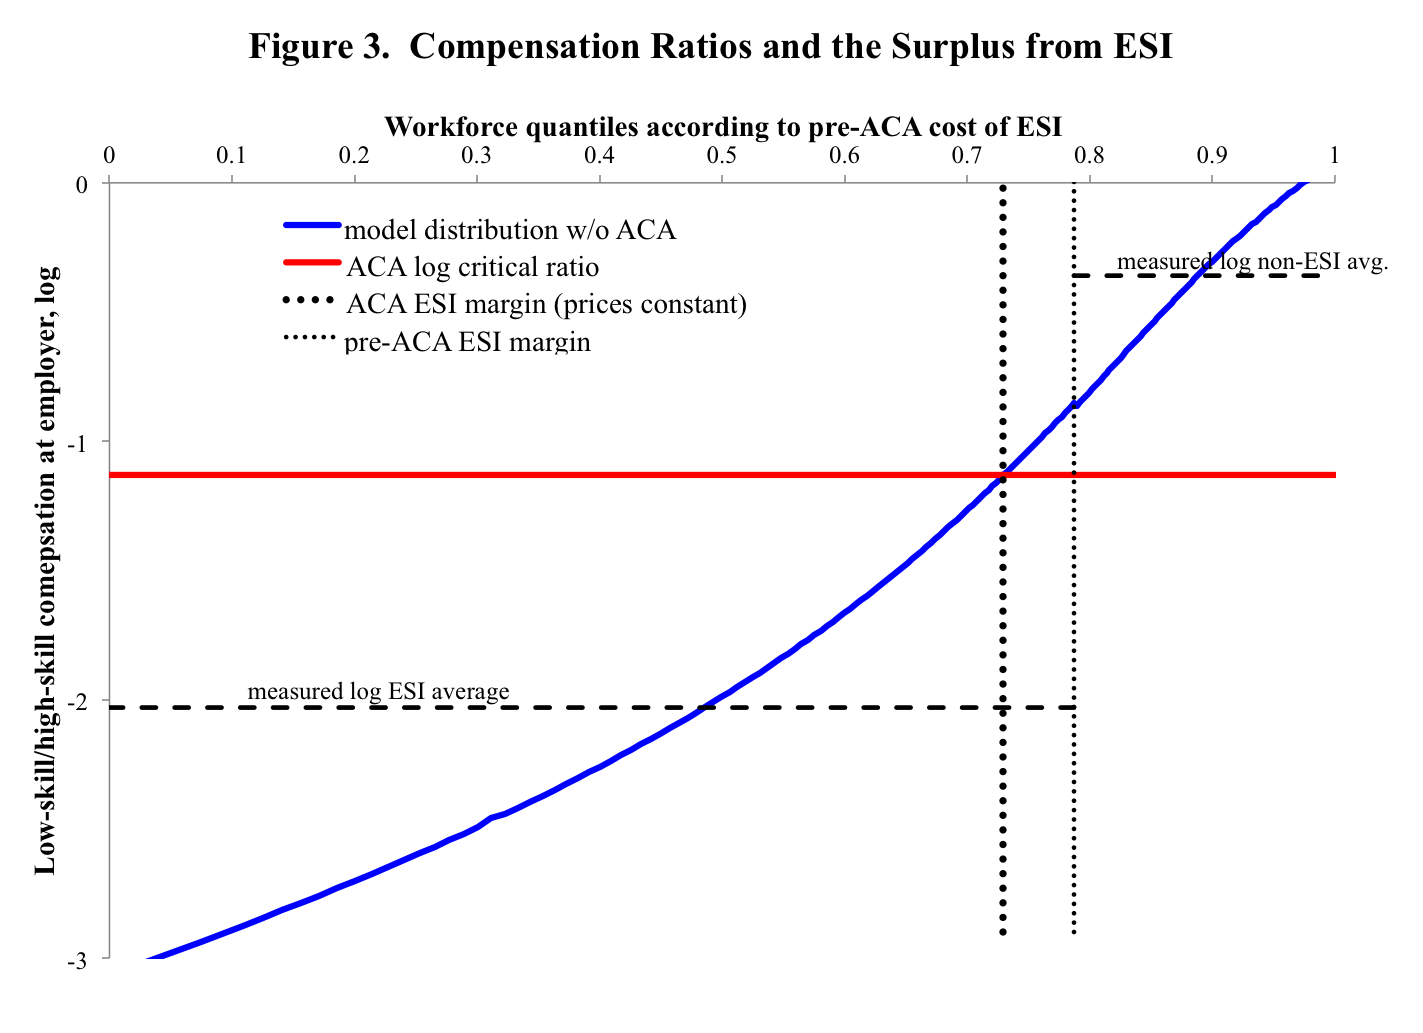
\includegraphics[scale=0.42]{CompensationRatios.png}
\end{figure}
\end{frame}

\begin{frame}
\frametitle[alignment=center]{Gallen \& Mulligan 2016: Matching Moments-II}
\begin{figure}
\centering
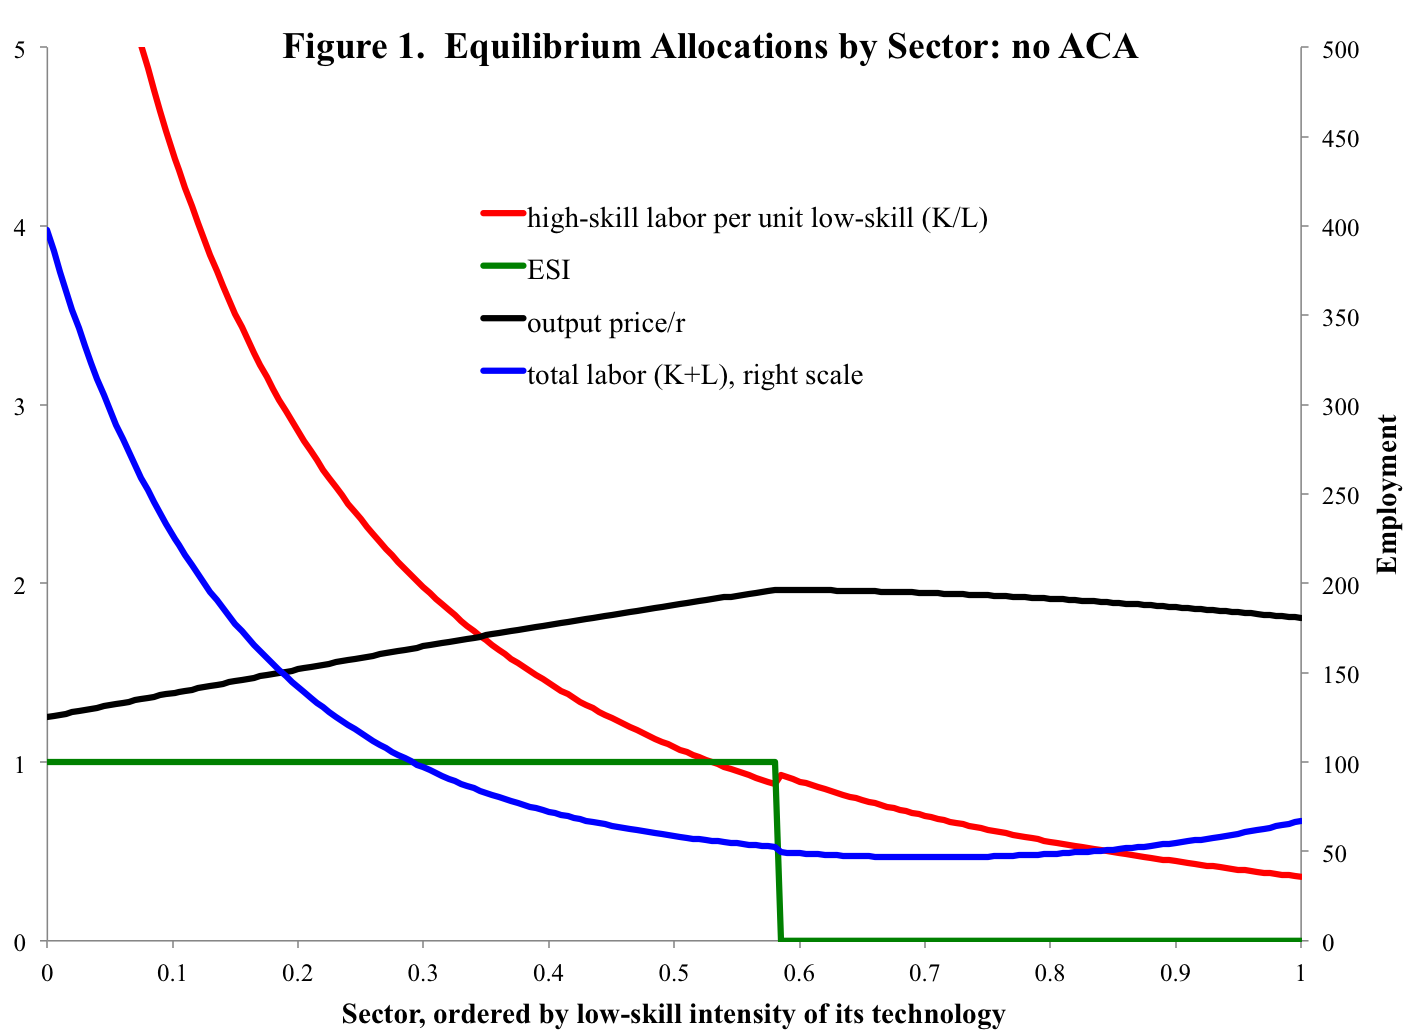
\includegraphics[scale=0.42]{Fig1.png}
\end{figure}
\end{frame}

\begin{frame}
\frametitle[alignment=center]{Gallen \& Mulligan 2016: Matching Moments-II}
\begin{figure}
\centering
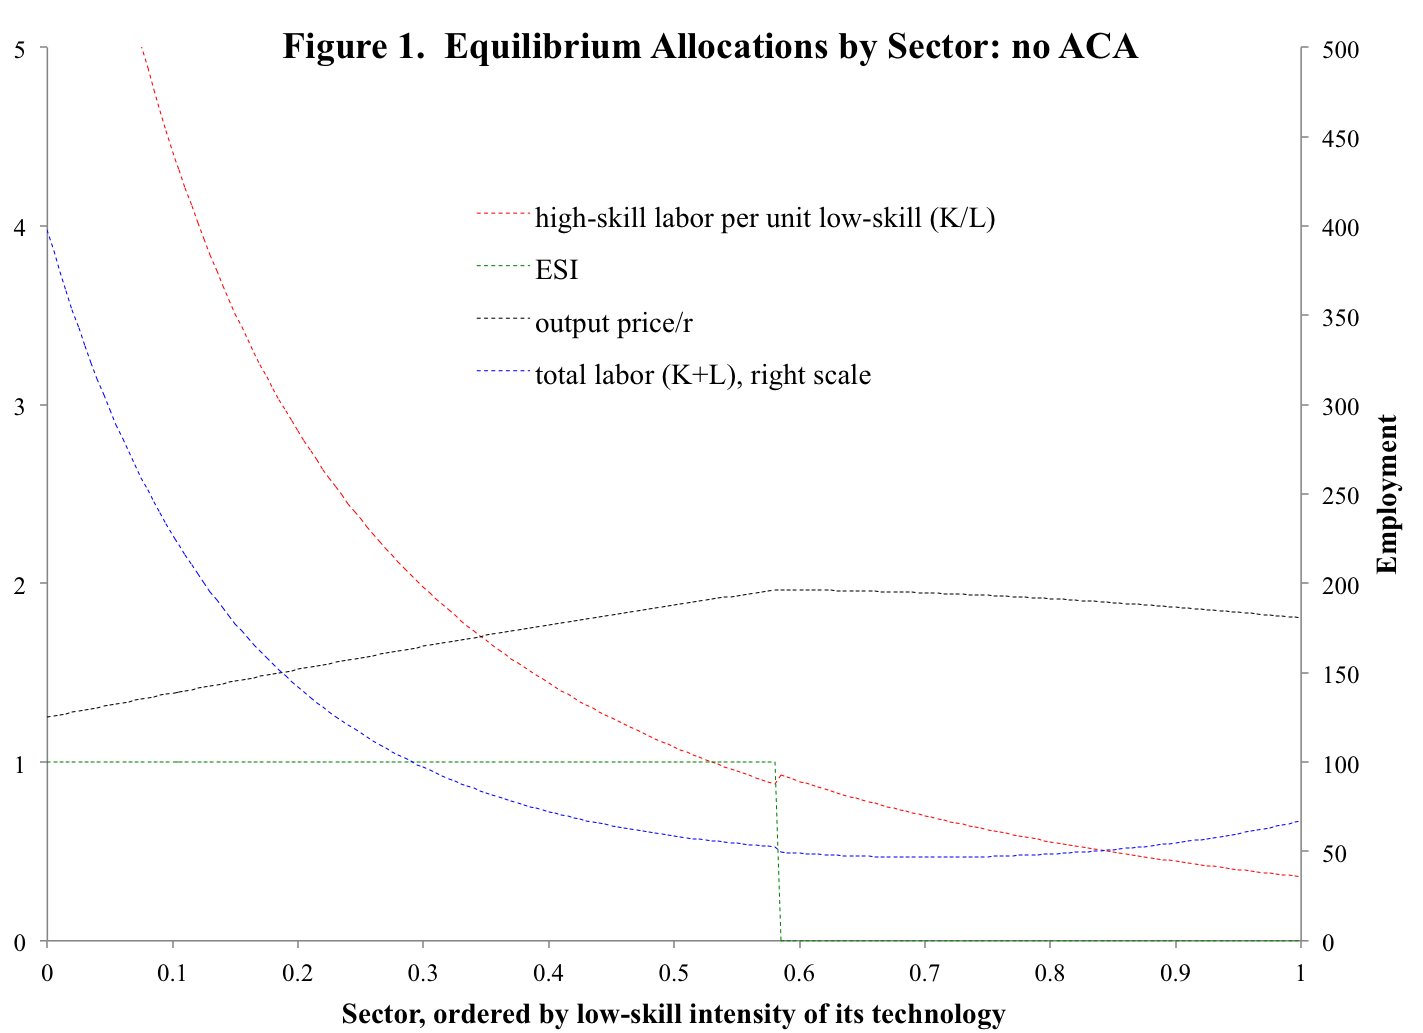
\includegraphics[scale=0.42]{Fig2.png}
\end{figure}
\end{frame}

\begin{frame}
\frametitle[alignment=center]{Gallen \& Mulligan 2016: Results-I\ \\ \ }
\begin{figure}
\centering
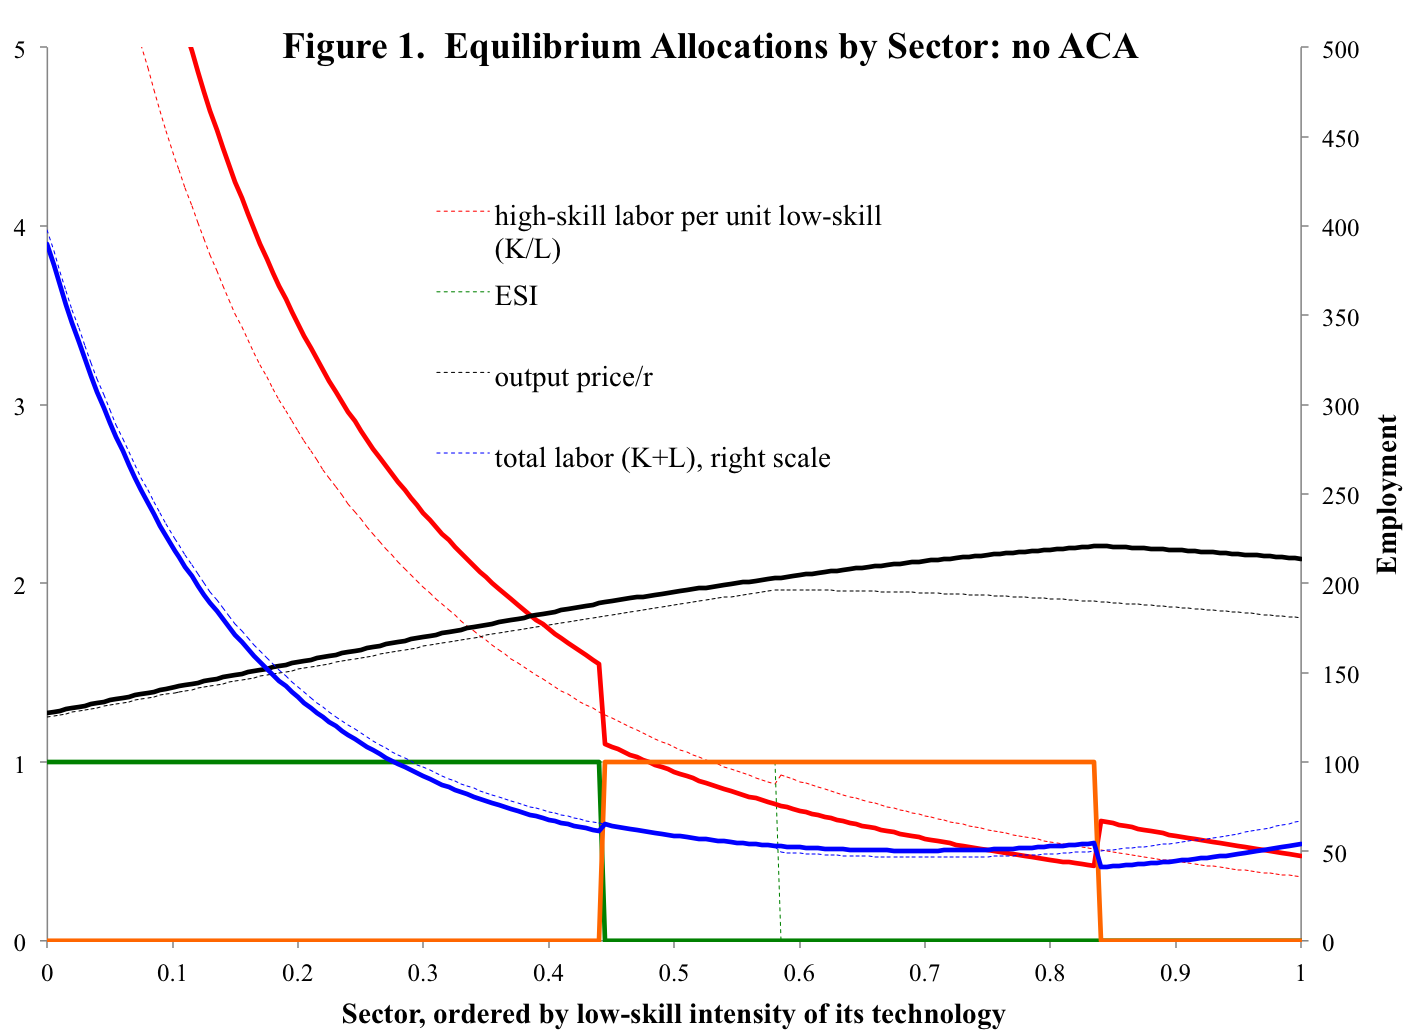
\includegraphics[scale=0.42]{Fig3.png}
\end{figure}
\end{frame}

\begin{frame}
\frametitle[alignment=center]{Gallen \& Mulligan 2016: Results-II}
\begin{figure}
\centering
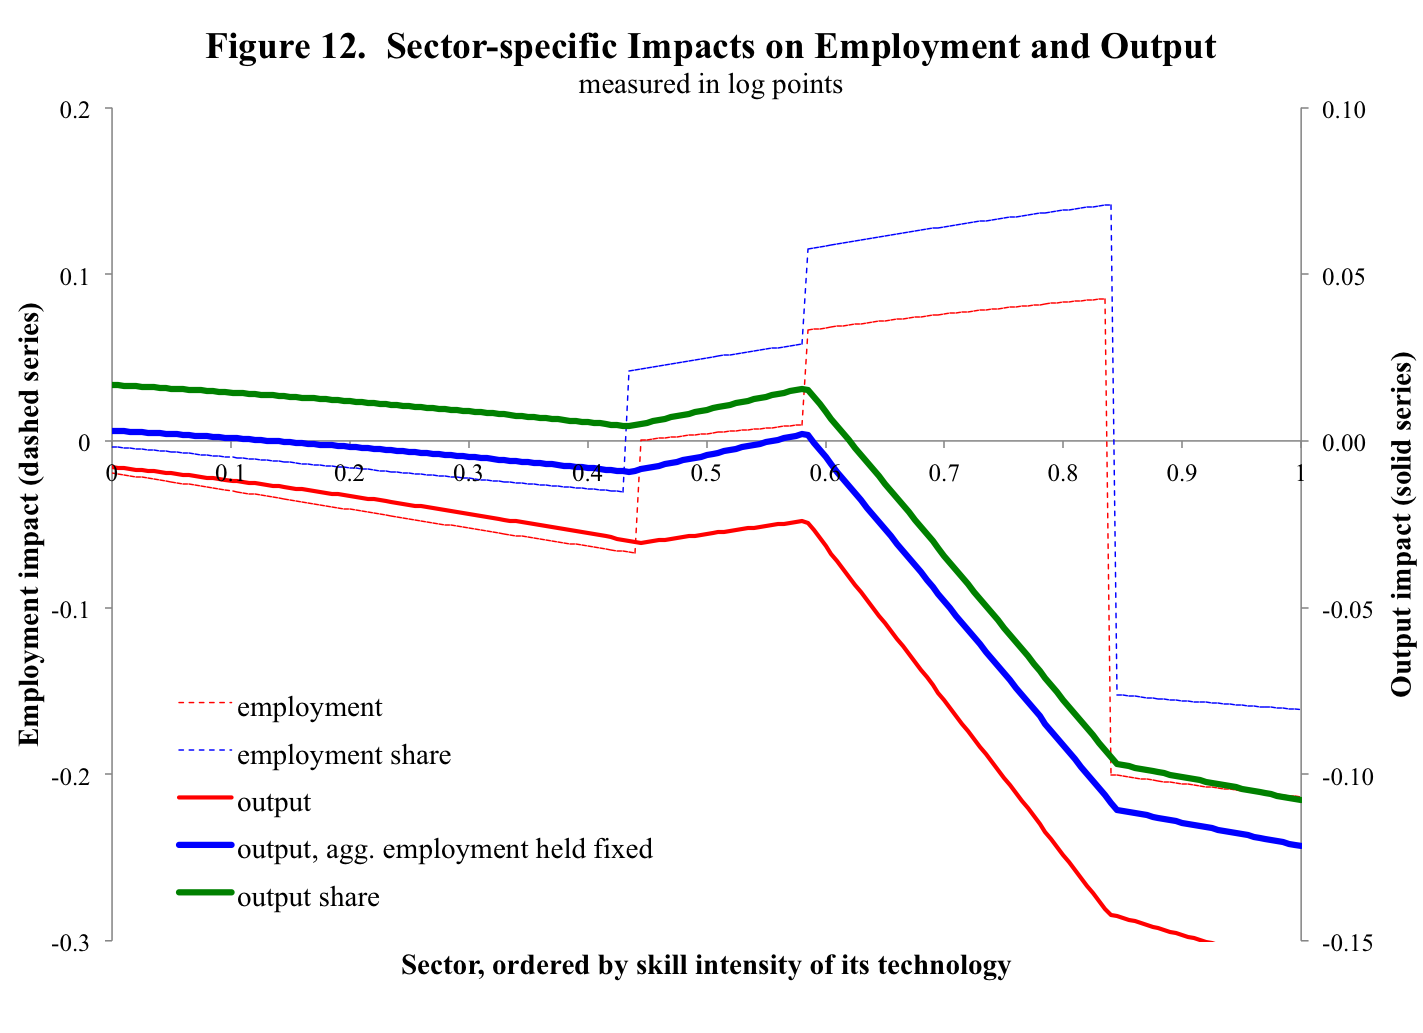
\includegraphics[scale=0.42]{OutputEffects.png}
\end{figure}
\end{frame}

\begin{frame}
\frametitle[alignment=center]{Gallen \& Mulligan 2016: Results-II}
\begin{figure}
\centering
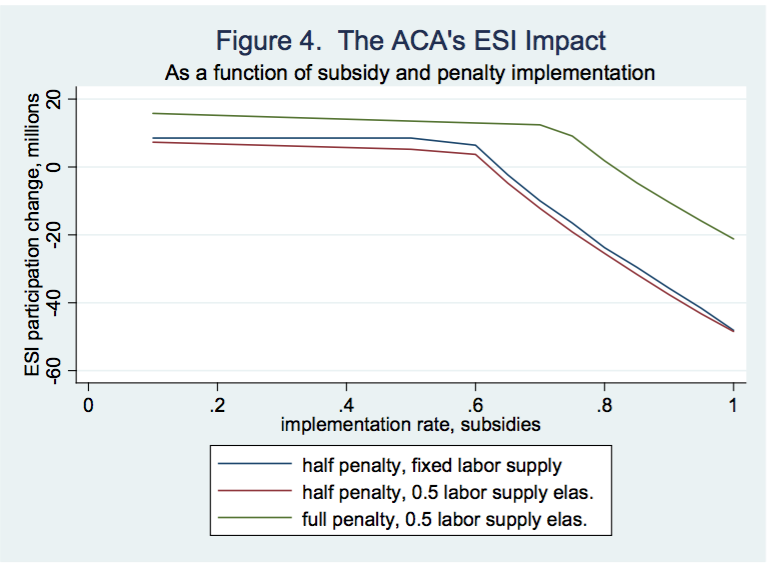
\includegraphics[scale=0.37]{ACAESIImpact.png}
\end{figure}
\end{frame}


\begin{frame}
\frametitle[alignment=center]{Gallen \& Mulligan 2016: Results}
\begin{itemize}
\item Less ESI, as $\sim$8\% of firms drop out of ESI
\item A lot less low-skill ESI, as low-skill (non-ESI) firms become more intensive in low-skill workers
\item More high-skill ESI, as high-skill (ESI) firms become more intensive in high-skill workers
\item $\sim3\%$ less working hours, as low-skill step out of labor force
\item $\sim$2\% less output, as firms skill mix becomes distorted and low-skill step out of work
\item 20 million people (10 million workers) leave ESI
\item Effects are \emph{extremely} nonlinear, depend on implementation rate
\end{itemize}
\end{frame}


\begin{frame}
\frametitle[alignment=center]{Why CGE?}
\begin{itemize}
\item<1-> Firms, workers are making a \emph{joint} decision
\bigskip
\item<2-> Workers in one sector impact workers from another sector
\bigskip
\item<3-> Normally, we might not care about this, but differential rewards are dramatic!
\bigskip
\item<4-> Any elasticity of substitution (and difference) and you're cooking with gas
\bigskip
\item<5-> Some industries ``win," some industries ``lose"
\bigskip
\item<6-> Calibration is important!  Massachusetts is high skill state with primarily high skill industries
\end{itemize}
\end{frame}


\end{document}